% Overleaf: upload this file together with nips15submit_e.sty and the figures/ folder (fig_loss.pdf, fig_h1.pdf,
% fig_h2.pdf, fig_linattn.pdf); compile with pdfLaTeX.
\documentclass{article}
\usepackage{nips15submit_e,times}
\nipsfinalcopy
\usepackage[utf8]{inputenc}
\usepackage[T1]{fontenc}
\usepackage{amsmath,amssymb}
\usepackage{graphicx}
\usepackage{booktabs}
\usepackage{multirow}
\usepackage{xcolor}
\usepackage{algorithm}
\usepackage[noend]{algpseudocode}
\usepackage{tikz}
\usetikzlibrary{positioning,arrows.meta,fit}
\usepackage[numbers,sort&compress]{natbib}
\usepackage[colorlinks=true,linkcolor=blue!50!black,citecolor=blue!50!black,urlcolor=blue!50!black]{hyperref}
\usepackage{microtype}
\usepackage{placeins}

\newcommand{\E}{\mathbb{E}}
\newcommand{\R}{\mathbb{R}}
\newcommand{\todo}[1]{\textcolor{red}{[#1]}}
\newcommand{\inprog}[1]{\textcolor{orange!70!black}{[In progress: #1]}}

\title{How Optimizers Shape In-Context Learning}

\author{
Jonah Cha \quad Kevin Chu \quad Ethan Dao \quad Isabella Hu\\
University of California, Berkeley\\
CS 182 final project
}

\begin{document}
\maketitle

\begin{abstract}
In-context learning (ICL) lets a transformer learn a new task from examples in its prompt without changing its weights. Prior work explains ICL's emergence through data and architecture, but the role of the optimizer that trains the weights is largely unexplored. We train a GPT-2-style transformer and a one-layer linear-attention model on in-context linear regression with SGD, AdamW and Muon. Comparing the optimizers at the same in-distribution error, we measure how well the model handles each input direction and which in-context algorithm it most resembles. With SGD and Adam the model learns the input directions one at a time, like principal component regression (PCR); with Muon its predictor departs from PCR, becoming ridge-like in linear attention and cutting off the weak directions more softly in a GPT-2-style model. Shifting test queries toward input directions that were rare or common in training, we find that Muon helps on rare directions and hurts on common ones, and a knob that flattens Muon's update spectrum by degrees shows, in linear attention, that this flattening drives the difference. The optimizer changes not only how fast ICL emerges, but also which in-context algorithm is learned.
\end{abstract}

\section{Introduction and background}
\label{sec:intro}
\paragraph{When ICL emerges.} \citet{garg2022} trained transformers on isotropic inputs, achieving near-least-squares performance on unseen linear functions. When test inputs instead varied much more in some directions than others, giving the model additional input--output examples of the same function eventually stopped reducing its prediction error on a new input. Least squares continued to improve using those same examples. In their test, the input covariance had eigenvalues proportional to $1/i^2$ in a random basis, and the model's error tracked least squares up to about ten examples and then plateaued, whereas noiseless least squares becomes exact once there are as many examples as dimensions. They also tested inputs from a low-dimensional subspace, noisy labels, rescaled prompts and queries in a different orthant from the examples, and found that bigger models reduced the error under these shifts considerably. They trained a GPT-2 \citep{radford2019gpt2} with Adam (learning rate $10^{-4}$, batch 64, 500,000 steps) and a curriculum over input dimension and prompt length. We take their model size, input dimension, prompt length and batch size, but put the same uneven input variances into training and vary the optimizer.

Which algorithm a trained model runs can be read off by comparing its predictions with reference algorithms \citep{akyurek2023}. Akyürek et al.\ constructed transformers that implement gradient descent and closed-form ridge regression, and found that in noiseless regression trained models moved from one step of gradient descent (one layer) through ridge regression to least squares (eight or more layers) as depth grew. \citet{bai2023} constructed transformers that implement least squares, ridge, Lasso, generalized linear models and gradient descent in context, and showed that one transformer can choose a different algorithm for each prompt. For large widths and depths the trained models approach Bayes-optimal estimators. A transformer can therefore represent many in-context algorithms, so which one a trained model runs depends on how it was trained. We use the same comparison, with principal component and ridge regression as references, because these are the two natural estimators when input directions differ in variance.

\citet{olsson2022} linked ICL in language models to induction heads, which form in an abrupt phase change visible as a bump in the loss: a short window early in training in which in-context learning improves sharply. \citet{raventos2023} found a task-diversity threshold: below it, a transformer acts as the Bayes estimator for its finite pretraining tasks; above it, it behaves like ridge regression and solves unseen tasks. Ridge corresponds to a Gaussian prior over all tasks, so above the threshold the model departs from the Bayes-optimal estimator for its own pretraining distribution. More weight decay lowered the threshold, while more layers or a larger embedding raised it, so training choices move which estimator emerges. \citet{singh2023} showed that emergent ICL can be transient, giving way to in-weights learning with continued training in their setting, synthetic few-shot classification, even while the training loss keeps falling; L2 regularization made ICL more persistent. Raventós et al.\ and Singh et al.\ trained with Adam, and Singh et al.\ list other optimizers as future work.

\paragraph{What attention computes, and how training gets there.} \citet{vonoswald2023} showed that a trained linear self-attention layer computes one step of gradient descent on the regression problem in its prompt. When input directions differ in variance, the best one-layer linear attention instead takes a step that divides each direction by its variance, with a correction for the finite number of examples that acts like a ridge penalty \citep{ahn2023}, and training reaches this solution \citep{zhang2023trained}. This end point shrinks the weak directions smoothly, as ridge regression does; it gives the optimal gains $\rho_j^\star$ we use as a reference in linear attention (Section~\ref{sec:methods}). The input distribution shapes the learned algorithm more than the targets do \citep{mahankali2023}. \citet{zhang2023trained} also shifted the test inputs: the trained layer tolerates some shifts but not a rescaling of all inputs, and GPT-2 models of Garg et al.'s size were more robust. Our query-shift test is similar, but compares optimizers at the same in-distribution error. More broadly, linear attention, state-space models and softmax attention can all be seen as solving a regression problem in the forward pass, with plain linear attention taking a single gradient step \citep{wang2025testtime}.

These results describe the end point of training or what an architecture can represent; optimizers differ in the path. \citet{zhang2025training} analysed linear attention's training dynamics on this task: merged key--query weights learn in one abrupt drop, while separate ones learn one principal input direction at a time, so that a model stopped early approximately runs principal component regression (PCR) on a growing set of directions. Training goes from saddle to saddle, direction $m$ takes time proportional to $\lambda_m^{-2}$, each drop lowers the loss by about $\lambda_m$, and both parametrizations end at the same solution; one-layer softmax attention with separate rank-one keys and queries shows the same stages. This variance-ordered learning mirrors the exact solutions of \citet{saxe2014} for deep linear networks, in which input--output modes are learned in order of their strength. PCR uses the strongest directions fully and ignores the rest; ridge regression uses every direction, shrinking the weak ones more.

\paragraph{How optimizers shape learning.} SGD, Adam and Shampoo \citep{gupta2018shampoo} can be read as steepest descent under different norms \citep{bernstein2024old}. Without its moving averages Adam becomes sign descent, steepest descent under the $\ell_\infty$ norm of the parameters, and Shampoo becomes spectral descent, the update $-\eta\,UV^\top$ for a gradient $G = USV^\top$, which is steepest descent under the spectral norm. Muon \citep{jordan2024muon} applies this spectral step to the momentum of each hidden weight matrix, approximating $UV^\top$ with a few Newton--Schulz iterations and leaving embeddings, output head, gains and biases to AdamW. Adding decoupled weight decay and matching the update size across matrix shapes lets Muon scale to language-model pretraining with about twice AdamW's compute efficiency \citep{liu2025muon}. AdamW itself is Adam with weight decay decoupled from the gradient update \citep{loshchilov2019}; we set the decay to zero, so that no arm has an explicit regularizer, because weight decay alone moves which estimator emerges \citep{raventos2023}. \citet{xie2025adam} showed that Adam's advantage depends on the coordinate axes: rotating GPT-2's parameter-space objective slowed Adam sharply, below even a rotation-equivariant SGD variant, while SGD is unaffected by such rotations. On language data, gradient descent makes slow progress on rare classes where Adam and sign descent are much less affected \citep{kunstner2024heavy}; by analogy one might expect AdamW to have learned more of the weak input directions than SGD at the same error, but SGD has learned at least as much (Table~\ref{tab:h1}).

Several recent analyses ask which directions spectral optimizers learn first. \citet{ma2026} proved that simplified Muon trains linear transformers on in-context regression at a rate independent of the condition number, unlike gradient descent and SignGD. \citet{dragutinovic2026} showed that simplified Muon trades gradient descent's simplicity bias for speed in linear models and in linear attention on this task, where it learns every principal direction at the same rate (head $i$ finishes in time proportional to $\lambda_i^{-1/3}$ rather than one after another), with worse generalization in experiments where tasks shared structure, including a two-layer softmax transformer on a cycle task. By contrast, \citet{vasudeva2025} and \citet{wang2025muon} found that this more even learning helps spectral optimizers on rare classes: spectral descent learns all principal components of Gaussian-mixture data at equal rates, which improves class-balanced loss early in training, a gap that persists when gradient descent uses normalized step sizes and that depth amplifies. In language models, most of Muon's advantage over Adam sits in the attention value/output weights and the MLPs, and in a one-layer associative memory with imbalanced classes Muon learns all classes evenly while Adam's errors can be very uneven. The even learning is fragile: small-batch gradient noise pushes Muon's update back toward the gradient and restores strongest-directions-first learning in deep linear networks \citep{jacobs2026}, and depth amplifies the separation between modes. This matters here because we train with batches of 64. \citet{dong2026muonp} and \citet{shumaylov2026} studied updates that flatten the singular values only partly, judging them by loss and downstream accuracy; Shumaylov et al.\ found that these barely depend on the update's spectrum, since replacing the singular values with random noise matches Muon. Dong and Sawin's update raises the singular values to a power $p$, interpolating between gradient descent ($p=1$) and Muon ($p=0$); it helps most in fine-tuning, while full flattening remains better for pretraining. We use the same knob to ask what the spectrum does to the learned algorithm rather than to the loss.

These optimizer studies motivate comparing learning under imbalanced training inputs, while Garg's result motivates testing robustness when the input distribution changes at evaluation.

\paragraph{Contributions.} The analyses above study simplified Muon (no momentum, exact orthogonalization) in linear models, linear attention or associative memories, mostly in the gradient-flow or full-batch limit, and judge optimizers mostly by speed or loss. We train SGD, AdamW and full Muon on in-context linear regression whose inputs vary much more in some directions than others, in a GPT-2 of Garg et al.'s size and in one-layer linear attention. We compare the optimizers at the same in-distribution error, to see how each spreads its remaining error across input directions, and measure how well the model handles each direction and which in-context algorithm it most resembles. We shift test queries toward input directions that were rare or common in training to test when Muon helps out of distribution and when it hurts, and use a knob that flattens Muon's update spectrum by degrees to test why. Muon needs about three times fewer training steps and, at the same error, its in-context predictor is less PCR-like; out of distribution it helps on rare directions and hurts on common ones; and in linear attention, flattening the update is what makes the difference.

\section{Methods}
\label{sec:methods}

\subsection{Task and models}
Each prompt is a sequence $(x_1, y_1, \dots, x_n, y_n, x_q)$ with $n = 40$ examples and a query, $y_i = w^\top x_i$, a fresh task $w \sim \mathcal N(0, I_d)$ per prompt and inputs $x \sim \mathcal N(0, \Lambda)$ in $d = 20$ dimensions, with
\begin{equation}
\Lambda = \mathrm{diag}(\lambda_1,\dots,\lambda_d), \qquad \lambda_j \propto 1/j^2, \qquad \textstyle\sum_j \lambda_j = d .
\end{equation}
The strongest input direction has 400 times the variance of the weakest, and the top two carry 78\% of the total. We measure error after all 40 examples on 1,000 held-out prompts,
\begin{equation}
\mathrm{err} = \tfrac{1}{d}\,\E\big[(\hat y - y)^2\big],
\label{eq:err}
\end{equation}
which is 1 for predicting zero. Models are trained on the squared error of every prediction in a fresh batch of 64 prompts per step, so training loss estimates the population loss.

\textbf{GPT-2.} We use the 12-layer, 8-head, width-256 GPT-2 of \citet{garg2022} (9.5M parameters). Each example becomes two tokens, $[x_i, 0]$ and $[x_i, y_i]$, and the model predicts $y_i$ at $[x_i, 0]$ from the earlier examples (Figure~\ref{fig:setup}).

\textbf{Linear attention.} To vary the optimizer finely, we also train the one-layer, 8-head linear-attention model of \citet{zhang2025training} ($d = 8$, $N = 32$ examples). It predicts $\hat y = h^\top \Gamma x_q$, where $h = \frac1N\sum_n y_n x_n$ summarizes the examples and $\Gamma$ is a learned $d \times d$ matrix (the sum of the heads' key--query products), so its loss can be computed exactly. For each direction $j$ we report the fraction of the optimal gain the model has learned, $\rho_j/\rho_j^\star$ with $\rho_j = \lambda_j \Gamma_{jj}$: 1 means direction $j$ is used as well as the best one-layer model uses it, and 0 means it is ignored (Appendix~\ref{app:small}).

\begin{figure}[!t]
\centering
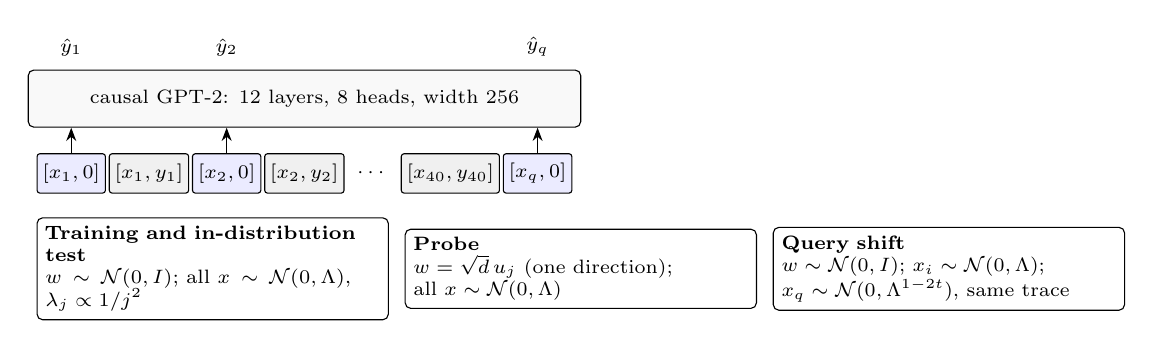
\begin{tikzpicture}[
  tok/.style={draw, rounded corners=1pt, minimum height=5mm, inner sep=2pt, font=\scriptsize},
  qt/.style={tok, fill=blue!8}, ct/.style={tok, fill=gray!12},
  box/.style={draw, rounded corners=2pt, align=left, font=\scriptsize, inner sep=3pt, text width=4.25cm},
  >=Stealth]
\node[qt] (a1) {$[x_1,0]$};
\node[ct, right=1pt of a1] (b1) {$[x_1,y_1]$};
\node[qt, right=1pt of b1] (a2) {$[x_2,0]$};
\node[ct, right=1pt of a2] (b2) {$[x_2,y_2]$};
\node[font=\scriptsize, right=1pt of b2] (dots) {$\cdots$};
\node[ct, right=1pt of dots] (bn) {$[x_{40},y_{40}]$};
\node[qt, right=1pt of bn] (aq) {$[x_q,0]$};
\node[draw, fill=gray!5, rounded corners=2pt, fit=(a1)(aq), inner sep=3pt, yshift=9.5mm, minimum height=5.5mm,
      font=\scriptsize, label={[font=\scriptsize]center:causal GPT-2: 12 layers, 8 heads, width 256}] (gpt) {};
\foreach \t/\lab in {a1/{$\hat y_1$}, a2/{$\hat y_2$}, aq/{$\hat y_q$}} {
  \draw[->] (\t.north) -- (\t.north |- gpt.south);
  \node[font=\scriptsize, above=0.5mm of \t.north |- gpt.north] {\lab};
}
\node[box, below=3mm of a1.south west, anchor=north west] (train) {\textbf{Training and in-distribution test}\\ $w\sim\mathcal N(0,I)$; all $x\sim\mathcal N(0,\Lambda)$, $\lambda_j\propto 1/j^2$};
\node[box, right=2mm of train] (probe) {\textbf{Probe}\\ $w=\sqrt d\,u_j$ (one direction);\\ all $x\sim\mathcal N(0,\Lambda)$};
\node[box, right=2mm of probe] (shift) {\textbf{Query shift}\\ $w\sim\mathcal N(0,I)$; $x_i\sim\mathcal N(0,\Lambda)$;\\ $x_q\sim\mathcal N(0,\Lambda^{1-2t})$, same trace};
\end{tikzpicture}
\caption{\textbf{How a prompt is fed to the model, and the three kinds of test prompts.} Each example becomes two tokens: $[x_i,0]$ (blue), where the model predicts $y_i$, and $[x_i,y_i]$ (grey). The probe uses a task along a single input direction $j$; the query shift changes only the distribution of the final query.}
\label{fig:setup}
\end{figure}

\subsection{Optimizers}
\textbf{SGD} uses heavy-ball momentum 0.9 and gradient clipping at norm 1; \textbf{AdamW} \citep{kingma2015adam,loshchilov2019} uses $\beta = (0.9, 0.999)$ and no weight decay. \textbf{Muon} \citep{jordan2024muon} replaces the momentum update $M = USV^\top$ of each weight matrix by an approximation of its polar factor $UV^\top$, computed with five Newton--Schulz iterations (Algorithm~\ref{alg:muon}). Every singular value is set to about one, so every singular direction of the update moves by approximately the same amount. Muon trains all weight matrices in the transformer blocks; AdamW trains the remaining 0.7\% of parameters.

\begin{algorithm}[t]
\caption{Muon update for one weight matrix $W$ (Nesterov momentum and shape scaling as in \citet{jordan2024muon} omitted)}
\label{alg:muon}
\begin{algorithmic}[1]
\Require gradient $G$, momentum $M$ (initially 0), learning rate $\eta$, $\mu = 0.95$
\State $M \gets \mu M + G$ \Comment{momentum}
\State $X \gets M / \|M\|_F$
\State \textbf{repeat 5 times:} $X \gets aX + b\,XX^\top X + c\,(XX^\top)^2 X$ \Comment{pushes every singular value toward 1, so $X \approx UV^\top$}
\State $W \gets W - \eta X$
\end{algorithmic}
\end{algorithm}

\textbf{Spectral knob.} To test whether flattening the singular values is what matters, we replace lines 2--3 of Algorithm~\ref{alg:muon} by an exact SVD that keeps a power $p$ of the singular values,
\begin{equation}
M = U S V^\top \;\longmapsto\; c\, U S^{p} V^\top ,
\label{eq:knob}
\end{equation}
where $c$ rescales the update to a fixed size. At $p = 1$ the update keeps the gradient's shape (momentum SGD with a normalized step), at $p = 0$ every singular value is 1 (exact orthogonalization, as in Muon), and values in between flatten partly \citep{dong2026muonp}. We run $p \in \{1, 0.75, 0.5, 0.25, 0.1, 0\}$ in linear attention and $p \in \{1, 0\}$ at Garg scale.

\subsection{Measurements}
\label{sec:measure}
\textbf{Matched error.} Muon needs about three times fewer training steps, so we compare optimizers at equal in-distribution error (0.04, which we verified at 0.05 and 0.03), interpolating every measurement between evaluations. This shows how each optimizer spreads its remaining error across input directions.

\textbf{Probe score.} For each direction $j$ we give the model prompts whose task points along $u_j$ alone and score $f_j = 1 - \sum(\hat y - y)^2/\sum y^2$, averaged over predictions made with 16 to 40 examples. $f_j = 1$ means that direction $j$ has been learned. A predictor that ignores direction $j$, as PCR does, scores below zero, because it fits $y$ with the other directions; ridge regression never does. We report the mean $\bar f$ over directions 3--20 and the bounded score $\bar f_+$, the mean of $\max(f_j, 0)$, which counts only what is learned.

\textbf{Which algorithm.} We also compare the model's predictions with two families of reference estimators computed from the same context $(X, y)$,
\begin{align}
\text{ridge:}\quad \hat w &= \arg\min_w \|Xw - y\|^2 + \alpha\|w\|^2, \\
\text{PCR}_m:\quad \hat w &= \arg\min_{w \in \mathrm{span}(u_1,\dots,u_m)} \|Xw - y\|^2,
\end{align}
where $X$ stacks the context inputs as rows and $y$ their labels; both predict $\hat y = x_q^\top \hat w$. Ridge uses every direction but shrinks the weak ones; PCR$_m$ uses only the top $m$ directions and ignores the rest (in practice we add a small ridge penalty). We report the distance to the nearest member of each family. In linear attention we fit a PCR step and a ridge curve directly to the gain profile and report the ratio of their residuals (above 1: closer to ridge).

\textbf{Query shift.} We keep the task and the context and draw only the query from $\mathcal{N}(0, \Lambda^{1-2t})$ at the same total variance: $t<0$ shifts it toward high-variance (``common'') directions and $t>0$ toward low-variance (``rare'') ones.

\textbf{Controls and statistics.} Within a seed, every optimizer starts from the same initialization and sees the same training and evaluation prompts; only the optimizer and its learning rate change (Table~\ref{tab:hparams}, Appendix~\ref{app:lr}). Error bars are $\pm1$ standard deviation over five seeds at Garg scale, and min--max over three seeds in linear attention; comparisons are paired by seed.

\section{Results}
\label{sec:results}

\subsection{Training and validation loss}
Training and validation loss coincide (Figure~\ref{fig:loss}a), as every training prompt is new. Muon reaches each matched error in about three times fewer steps than AdamW (error 0.04 after about 600 steps, against about 2,000), Muon without flattening only slightly sooner than AdamW, and SGD last (Figure~\ref{fig:loss}b).

\begin{figure}[t]
\centering
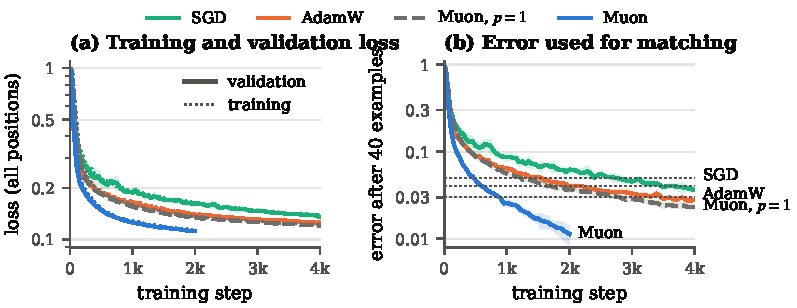
\includegraphics[width=\linewidth]{figures/fig_loss.pdf}
\caption{\textbf{Muon reaches every error level in about three times fewer steps than AdamW.} (a) Training (dotted) and validation (solid) loss. (b) Error after 40 examples; dotted horizontal lines mark the three errors at which we compare optimizers. Lines: mean of five seeds; shading: $\pm1$ standard deviation across seeds. Log scales, because the curves span two orders of magnitude.}
\label{fig:loss}
\end{figure}

\subsection{Which in-context algorithm: Muon's predictor is less PCR-like}
\label{sec:h1}

Figure~\ref{fig:h1}a shows how well each model has learned each input direction at error 0.04. Every optimizer learns the strong directions first, and all have learned about the first eleven. Beyond that point AdamW behaves like PCR: on the directions it has not learned, its predictions are as poor as those of PCR, which ignores them. Muon's cutoff is softer, with predictions that degrade gradually over directions 12--15. Muon's probe score is higher than AdamW's in every seed (Table~\ref{tab:h1}, Figure~\ref{fig:h1}b), and its predictions are farther from the nearest PCR estimator in every seed and at every matched error. SGD lies between the two. The optimizers have learned similar amounts of the weak directions (amount learned, Table~\ref{tab:h1}); they differ in how the predictor treats the directions it has not learned. One-step gradient descent, plain or preconditioned, is about ten times farther from every model than PCR or ridge, so these two are the relevant references. In linear attention the same split is sharper: SGD and Adam are PCR-like and Muon is ridge-like (Section~\ref{sec:h3}).

\begin{figure}[t]
\centering
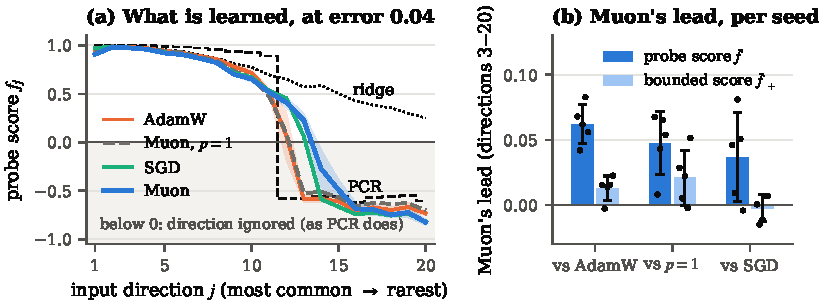
\includegraphics[width=\linewidth]{figures/fig_h1.pdf}
\caption{\textbf{All optimizers learn the strong directions first; Muon cuts off the weak ones more softly.} Garg-scale GPT-2, compared at the same error (0.04). (a) How well each input direction is learned: 1 = learned, below 0 = ignored (as PCR does). Black: PCR (dashed) and ridge regression (dotted) for reference. Shading: $\pm1$ standard deviation over five seeds. (b) Muon's lead over each optimizer, averaged over directions 3--20: on the probe score (dark) and on the bounded score that counts only what is learned (light). Dots: seeds.}
\label{fig:h1}
\end{figure}

\begin{table}[t]
\caption{\textbf{Muon's predictor is the least PCR-like} (Garg scale, error 0.04; mean $\pm$ s.d.\ over five seeds, averaged over directions 3--20). Probe score: higher means unlearned directions are not ignored. Amount learned: bounded score, which counts only what is learned. Distance to PCR: higher means less PCR-like. Last row: Muon minus AdamW, with the number of seeds where it is positive.}
\label{tab:h1}
\vspace{2pt}
\centering\small
\begin{tabular}{@{}lccc@{}}
\toprule
 & Probe score $\bar f$ & Amount learned $\bar f_+$ & Distance to PCR \\
\midrule
SGD & $0.16 \pm 0.03$ & $0.44 \pm 0.01$ & 0.024 \\
AdamW & $0.13 \pm 0.01$ & $0.43 \pm 0.01$ & 0.019 \\
Muon & $\mathbf{0.20 \pm 0.02}$ & $0.44 \pm 0.01$ & \textbf{0.027} \\
Muon, $p=1$ & $0.15 \pm 0.01$ & $0.42 \pm 0.02$ & 0.020 \\
\midrule
Muon $-$ AdamW & $+0.06$ (5/5 seeds) & $+0.01$ (4/5) & $+0.008$ (5/5) \\
\bottomrule
\end{tabular}
\end{table}

\subsection{Out of distribution: a trade-off}

Out of distribution, Muon trades a cost for a gain (Figure~\ref{fig:h2}). This follows from Figure~\ref{fig:h1}: shifting test queries toward rare directions rewards Muon's softer cutoff. On queries shifted toward high-variance directions its error is $1.3$--$1.8\times$ AdamW's in every seed; on queries shifted toward low-variance directions it is lower. The cost falls on errors that are already tiny ($+0.004$ on an error of 0.007), while the gain falls where every model is weakest ($-0.03$ on 0.83). Without flattening, neither effect appears.

\begin{figure}[t]
\centering
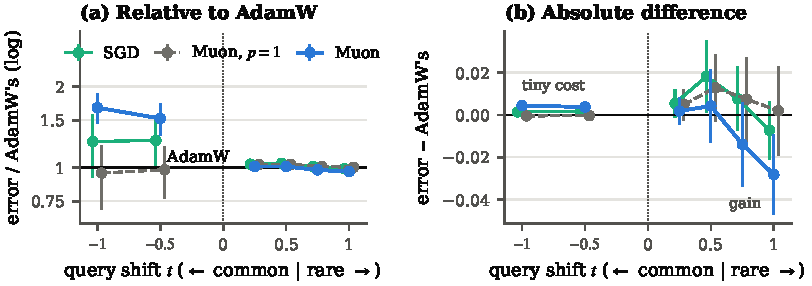
\includegraphics[width=\linewidth]{figures/fig_h2.pdf}
\caption{\textbf{Muon trades a tiny cost on common directions for a gain on rare ones.} Test queries are shifted toward directions that were common ($t<0$) or rare ($t>0$) in training. (a) Error relative to AdamW (log scale; 1 = same as AdamW). (b) Error minus AdamW's: the cost at $t<0$ is negligible in absolute terms, and the gain at $t>0$ is larger. Mean of five seeds; bars: $\pm1$ standard deviation.}
\label{fig:h2}
\end{figure}

\subsection{Why: spectral flattening}
\label{sec:h3}

Linear attention lets us vary the flattening power $p$ finely (Figure~\ref{fig:linattn}). With little or no flattening ($p \ge 0.25$) the learned predictor is PCR-like, like SGD's: it has learned the two strongest directions and little else. With full or near-full flattening ($p \le 0.1$) it spreads its gain over the weak directions and its profile becomes ridge-shaped, like Muon's. Flattening also brings the rare-ward gain out of distribution (Appendix~\ref{app:small}). At Garg scale, Muon without flattening ($p=1$) behaves like AdamW on every measure and loses most of its speed-up, while exact orthogonalization ($p=0$, one seed) behaves like Muon.

\begin{figure}[t]
\centering
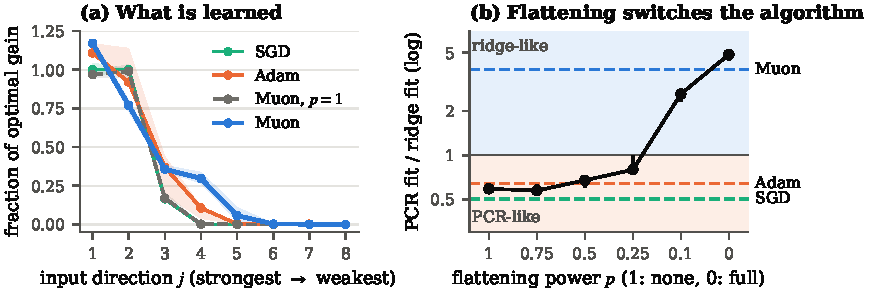
\includegraphics[width=\linewidth]{figures/fig_linattn.pdf}
\caption{\textbf{In linear attention, flattening Muon's update turns the learned gain profile from PCR-shaped (a step) to ridge-shaped (smooth).} (a) Fraction of the optimal gain learned per input direction: SGD, Adam and unflattened Muon mostly learn the two strongest directions, while Muon spreads gain over weaker ones. (b) PCR-versus-ridge score as Muon's update is flattened from $p=1$ (none) to $p=0$ (full); above 1 is ridge-shaped (log scale). Dashed lines: SGD, Adam and Muon. Median of three seeds; bands and bars: min--max.}
\label{fig:linattn}
\end{figure}

\FloatBarrier
\section{Discussion and conclusion}
\label{sec:discussion}

The optimizer changes not only how fast in-context learning emerges but which in-context algorithm the model runs on the way. SGD and AdamW follow the variance-ordered, PCR-like path that theory predicts for linear attention. Muon's spectral flattening lets the predictor move away from PCR: to a ridge-like predictor in linear attention, and to a softer cutoff in full transformers. Out of distribution this is a trade-off rather than a free gain, better on queries that emphasize rare directions and slightly worse on those that emphasize common ones. At equal steps Muon is simply further along. Larger batches, longer training and other input spectra are natural next tests.


\renewcommand{\bibfont}{\footnotesize}
\setlength{\bibsep}{1pt}
\begin{thebibliography}{29}
\providecommand{\natexlab}[1]{#1}
\providecommand{\url}[1]{\texttt{#1}}
\expandafter\ifx\csname urlstyle\endcsname\relax
  \providecommand{\doi}[1]{doi: #1}\else
  \providecommand{\doi}{doi: \begingroup \urlstyle{rm}\Url}\fi

\bibitem[Ahn et~al.(2023)Ahn, Cheng, Daneshmand, and Sra]{ahn2023}
Kwangjun Ahn, Xiang Cheng, Hadi Daneshmand, and Suvrit Sra.
\newblock Transformers learn to implement preconditioned gradient descent for
  in-context learning.
\newblock In \emph{Advances in Neural Information Processing Systems}, 2023.

\bibitem[Aky{\"u}rek et~al.(2023)Aky{\"u}rek, Schuurmans, Andreas, Ma, and
  Zhou]{akyurek2023}
Ekin Aky{\"u}rek, Dale Schuurmans, Jacob Andreas, Tengyu Ma, and Denny Zhou.
\newblock What learning algorithm is in-context learning? {I}nvestigations with
  linear models.
\newblock In \emph{International Conference on Learning Representations}, 2023.

\bibitem[Bai et~al.(2023)Bai, Chen, Wang, Xiong, and Mei]{bai2023}
Yu~Bai, Fan Chen, Huan Wang, Caiming Xiong, and Song Mei.
\newblock Transformers as statisticians: Provable in-context learning with
  in-context algorithm selection.
\newblock In \emph{Advances in Neural Information Processing Systems}, 2023.

\bibitem[Bernstein and Newhouse(2024)]{bernstein2024old}
Jeremy Bernstein and Laker Newhouse.
\newblock Old optimizer, new norm: An anthology.
\newblock \emph{arXiv preprint arXiv:2409.20325}, 2024.

\bibitem[Dong and Sawin(2026)]{dong2026muonp}
Yihe Dong and Will Sawin.
\newblock {M}uon$^p$: {M}uon with fractional spectral powers.
\newblock \emph{arXiv preprint arXiv:2606.13867}, 2026.

\bibitem[Dragutinovi{\'c} et~al.(2026)Dragutinovi{\'c}, Zhang, and
  Ranganath]{dragutinovic2026}
Sara Dragutinovi{\'c}, Yedi Zhang, and Rajesh Ranganath.
\newblock To use or not to use {M}uon: How simplicity bias in optimizers
  matters.
\newblock \emph{arXiv preprint arXiv:2603.00742}, 2026.

\bibitem[Garg et~al.(2022)Garg, Tsipras, Liang, and Valiant]{garg2022}
Shivam Garg, Dimitris Tsipras, Percy Liang, and Gregory Valiant.
\newblock What can transformers learn in-context? {A} case study of simple
  function classes.
\newblock In \emph{Advances in Neural Information Processing Systems}, 2022.

\bibitem[Gupta et~al.(2018)Gupta, Koren, and Singer]{gupta2018shampoo}
Vineet Gupta, Tomer Koren, and Yoram Singer.
\newblock Shampoo: Preconditioned stochastic tensor optimization.
\newblock In \emph{International Conference on Machine Learning}, 2018.

\bibitem[Jacobs and Burkholz(2026)]{jacobs2026}
Tom Jacobs and Rebekka Burkholz.
\newblock From parallel to sequential: Small-batch noise restores simplicity
  bias of {M}uon.
\newblock \emph{arXiv preprint arXiv:2610.16868}, 2026.

\bibitem[Jordan et~al.(2024)Jordan, Jin, Boza, You, Cesista, Newhouse, and
  Bernstein]{jordan2024muon}
Keller Jordan, Yuchen Jin, Vlado Boza, Jiacheng You, Franz Cesista, Laker
  Newhouse, and Jeremy Bernstein.
\newblock Muon: An optimizer for hidden layers in neural networks.
\newblock Blog post, \url{https://kellerjordan.github.io/posts/muon/};
  implementation at \url{https://github.com/KellerJordan/Muon}, 2024.

\bibitem[Kingma and Ba(2015)]{kingma2015adam}
Diederik~P. Kingma and Jimmy Ba.
\newblock Adam: A method for stochastic optimization.
\newblock In \emph{International Conference on Learning Representations}, 2015.

\bibitem[Kunstner et~al.(2024)Kunstner, Yadav, Milligan, Schmidt, and
  Bietti]{kunstner2024heavy}
Frederik Kunstner, Robin Yadav, Alan Milligan, Mark Schmidt, and Alberto
  Bietti.
\newblock Heavy-tailed class imbalance and why {A}dam outperforms gradient
  descent on language models.
\newblock \emph{arXiv preprint arXiv:2402.19449}, 2024.

\bibitem[Liu et~al.(2025)Liu, Su, Yao, et~al.]{liu2025muon}
Jingyuan Liu, Jianlin Su, Xingcheng Yao, et~al.
\newblock {M}uon is scalable for {LLM} training.
\newblock \emph{arXiv preprint arXiv:2502.16982}, 2025.

\bibitem[Loshchilov and Hutter(2019)]{loshchilov2019}
Ilya Loshchilov and Frank Hutter.
\newblock Decoupled weight decay regularization.
\newblock In \emph{International Conference on Learning Representations}, 2019.

\bibitem[Ma et~al.(2026)Ma, Huang, Chi, and Chen]{ma2026}
Jianhao Ma, Yu~Huang, Yuejie Chi, and Yuxin Chen.
\newblock Preconditioning benefits of spectral orthogonalization in {M}uon.
\newblock \emph{arXiv preprint arXiv:2601.13474}, 2026.

\bibitem[Mahankali et~al.(2024)Mahankali, Hashimoto, and Ma]{mahankali2023}
Arvind Mahankali, Tatsunori~B. Hashimoto, and Tengyu Ma.
\newblock One step of gradient descent is provably the optimal in-context
  learner with one layer of linear self-attention.
\newblock In \emph{International Conference on Learning Representations}, 2024.

\bibitem[Olsson et~al.(2022)Olsson, Elhage, Nanda, et~al.]{olsson2022}
Catherine Olsson, Nelson Elhage, Neel Nanda, et~al.
\newblock In-context learning and induction heads.
\newblock \emph{Transformer Circuits Thread}, 2022.

\bibitem[Radford et~al.(2019)Radford, Wu, Child, Luan, Amodei, and
  Sutskever]{radford2019gpt2}
Alec Radford, Jeffrey Wu, Rewon Child, David Luan, Dario Amodei, and Ilya
  Sutskever.
\newblock Language models are unsupervised multitask learners.
\newblock Technical report, OpenAI, 2019.

\bibitem[Ravent{\'o}s et~al.(2023)Ravent{\'o}s, Paul, Chen, and
  Ganguli]{raventos2023}
Allan Ravent{\'o}s, Mansheej Paul, Feng Chen, and Surya Ganguli.
\newblock Pretraining task diversity and the emergence of non-{B}ayesian
  in-context learning for regression.
\newblock In \emph{Advances in Neural Information Processing Systems}, 2023.

\bibitem[Saxe et~al.(2014)Saxe, McClelland, and Ganguli]{saxe2014}
Andrew~M. Saxe, James~L. McClelland, and Surya Ganguli.
\newblock Exact solutions to the nonlinear dynamics of learning in deep linear
  neural networks.
\newblock In \emph{International Conference on Learning Representations}, 2014.

\bibitem[Shumaylov et~al.(2026)Shumaylov, Da~Costa, Zaika, Mucsányi, Massucco,
  Gelberg, Schönlieb, Gal, and Hennig]{shumaylov2026}
Zakhar Shumaylov, Nathaël Da~Costa, Peter Zaika, Bálint Mucsányi, Alex
  Massucco, Yoav Gelberg, Carola-Bibiane Schönlieb, Yarin Gal, and Philipp
  Hennig.
\newblock {M}uon is not that special: Random or inverted spectra work just as
  well.
\newblock \emph{arXiv preprint arXiv:2605.11181}, 2026.

\bibitem[Singh et~al.(2023)Singh, Chan, Moskovitz, Grant, Saxe, and
  Hill]{singh2023}
Aaditya~K. Singh, Stephanie C.~Y. Chan, Ted Moskovitz, Erin Grant, Andrew~M.
  Saxe, and Felix Hill.
\newblock The transient nature of emergent in-context learning in transformers.
\newblock In \emph{Advances in Neural Information Processing Systems}, 2023.

\bibitem[Vasudeva et~al.(2025)Vasudeva, Deora, Zhao, Sharan, and
  Thrampoulidis]{vasudeva2025}
Bhavya Vasudeva, Puneesh Deora, Yize Zhao, Vatsal Sharan, and Christos
  Thrampoulidis.
\newblock How {M}uon's spectral design benefits generalization: A study on
  imbalanced data.
\newblock \emph{arXiv preprint arXiv:2510.22980}, 2025.

\bibitem[von Oswald et~al.(2023)von Oswald, Niklasson, Randazzo, Sacramento,
  Mordvintsev, Zhmoginov, and Vladymyrov]{vonoswald2023}
Johannes von Oswald, Eyvind Niklasson, Ettore Randazzo, Jo{\~a}o Sacramento,
  Alexander Mordvintsev, Andrey Zhmoginov, and Max Vladymyrov.
\newblock Transformers learn in-context by gradient descent.
\newblock In \emph{International Conference on Machine Learning}, 2023.

\bibitem[Wang et~al.(2025{\natexlab{a}})Wang, Shi, and Fox]{wang2025testtime}
Ke~Alexander Wang, Jiaxin Shi, and Emily~B. Fox.
\newblock Test-time regression: a unifying framework for designing sequence
  models with associative memory.
\newblock \emph{arXiv preprint arXiv:2501.12352}, 2025{\natexlab{a}}.

\bibitem[Wang et~al.(2025{\natexlab{b}})Wang, Zhang, Li, Du, Du, Pang, Yang,
  Hong, and Tan]{wang2025muon}
Shuche Wang, Fengzhuo Zhang, Jiaxiang Li, Cunxiao Du, Chao Du, Tianyu Pang,
  Zhuoran Yang, Mingyi Hong, and Vincent Y.~F. Tan.
\newblock {M}uon outperforms {A}dam in tail-end associative memory learning.
\newblock \emph{arXiv preprint arXiv:2509.26030}, 2025{\natexlab{b}}.

\bibitem[Xie et~al.(2024)Xie, Mohamadi, and Li]{xie2025adam}
Shuo Xie, Mohamad~Amin Mohamadi, and Zhiyuan Li.
\newblock Adam exploits $\ell_\infty$-geometry of loss landscape via
  coordinate-wise adaptivity.
\newblock \emph{arXiv preprint arXiv:2410.08198}, 2024.

\bibitem[Zhang et~al.(2024)Zhang, Frei, and Bartlett]{zhang2023trained}
Ruiqi Zhang, Spencer Frei, and Peter~L. Bartlett.
\newblock Trained transformers learn linear models in-context.
\newblock \emph{Journal of Machine Learning Research}, 2024.

\bibitem[Zhang et~al.(2025)Zhang, Singh, Latham, and Saxe]{zhang2025training}
Yedi Zhang, Aaditya~K. Singh, Peter~E. Latham, and Andrew Saxe.
\newblock Training dynamics of in-context learning in linear attention.
\newblock In \emph{International Conference on Machine Learning}, 2025.

\end{thebibliography}

\appendix
\section{Use of generative AI tools}
\label{app:ai}
\todo{TODO: to be written by the team.}

\section{Hyperparameters}
\label{app:lr}
\begin{table}[h]
\caption{\textbf{Settings and the reason for each} (Garg scale unless noted).}
\label{tab:hparams}
\vspace{2pt}
\centering\small
\begin{tabular}{@{}p{2.3cm}p{5.0cm}p{5.4cm}@{}}
\toprule
Setting & Value & Why \\
\midrule
Task & $d = 20$, $n = 40$, $\lambda_j \propto 1/j^2$ & \citet{garg2022}'s setting, with uneven input variances \\
Model & 12 layers, 8 heads, width 256 & \citet{garg2022} \\
Initialization & hidden weights $\mathcal{N}(0, 0.031^2)$ & With Garg et al.'s, SGD did not train \\
Training & batch 64, 4,000 steps, constant rate & Garg et al.'s batch; our compute budget \\
Seeds & 5 & Paired comparisons \\
SGD & lr 0.1, momentum 0.9, clipping at 1 & Learning-rate sweep; clipping prevents divergence \\
AdamW & lr $3\cdot10^{-4}$, weight decay 0 & Sweep; no explicit regularizer \\
Muon & lr 0.007, momentum 0.95 & Sweep; defaults of \citet{jordan2024muon} \\
Muon, $p=1$ & lr $5\cdot10^{-4}$ & Best of four rates \\
Linear attention & batch 1,024, 6,000 steps, 3 seeds, lr 0.02--0.03 & Setup of \citet{zhang2025training}; exact losses \\
Matched error & 0.04 (verified at 0.05 and 0.03) & Lowest error every optimizer reaches \\
\bottomrule
\end{tabular}
\end{table}

\textbf{How the learning rates were chosen.} SGD, AdamW and Muon rates come from sweeps on a smaller GPT-2 (seed 0), keeping the rate with the lowest area under the error curve on separate selection prompts. In linear attention each optimizer and each $p$ had its own six-point sweep on seed 0, selected by mean loss over training.

\textbf{Learning-rate check.} We trained seed 10 at Garg scale for 1,500 steps at rates about $3\times$ below and above each rate used and compared training loss. Each rate used is within 1.5\% of the best, and Muon's probe score at error 0.05 exceeds AdamW's for every pair of rates.

\section{Linear-attention details}
\label{app:small}
The optimal gain is $\rho_j^\star = \lambda_j N/((N+1)\lambda_j + \mathrm{tr}\,\Lambda)$ \citep{zhang2023trained}: close to 1 for strong directions and falling smoothly toward 0 for weak ones. We compare optimizers at the same excess loss $(L-L^\star)/(1-L^\star)$, where $L^\star$ is the loss of the optimal model. SGD here is plain gradient descent, as in \citet{zhang2025training}. The PCR/ridge residual ratio (median over seeds, averaged over excess losses 0.5 to 0.1) is 0.50 for SGD, 0.64 for Adam, 0.58--0.80 for $p \ge 0.25$, 2.62 at $p = 0.1$, 4.86 at $p = 0$ and 3.83 for standard Muon. Out of distribution, at excess loss 0.1, Muon's error is $1.15$--$1.20\times$ Adam's on common-ward queries and $0.95$--$0.97\times$ on rare-ward ones; the rare-ward ratio falls from about 1.02 at $p = 1$ to about 0.93 at $p = 0$.

\section{Reproducibility}
\label{app:repro}
Code, job files, training logs and checkpoints are at \url{https://github.com/MERC13/cs182finalproject}. The scripts in \texttt{scripts/} compute every figure and number in this paper from the committed logs (the README lists which script produces what).


\end{document}
